\chapter{Untersuchung des Laufzeitverhaltens}
Die Untersuchung des Laufzeitverhaltens wurde mithilfe eines Logik-
Analysers des Typs ''Agilent Logicwave E9340A'' durchgeführt. Dieser misst, wann und wie lange
ein Portpin gesetzt oder nicht gesetzt ist. Die Pins, die zur Durchführung
dieser Messungen nötig sind, dürfen noch nicht belegt sein. Vorteilhafterweise
besitzt die Platine zwei Ports, die noch nicht belegt sind, aber
trotzdem nach draußen gelegt wurden; somit konnte der Logik-Analyser
an die Platine angeschlossen und ein kleines Modul
geschrieben werden, um die Pins setzen und zurücksetzen zu
können. Diese Operationen wurden als Makros implementiert, um den
Mess-Overhead so gering wie möglich zu halten.
\begin{table}[htb]
\begin{center}
	\begin{tabular}{|c||c|c|}
		\hline
		\textbf{Makro} & \textbf{benötigte Takte} & \textbf{benötigte Zeit bei 16 MHz} \\ \hline \hline
		pin\_set() & 2 & 125 ns \\ \hline
		pin\_clear() & 2 & 125 ns \\ \hline
		pin\_toggle() & 4 & 250 ns \\ \hline
	\end{tabular}
	\caption{\label{pin_takte} Benötigte Takte/Zeit für Pin-Operationen}
\end{center}
\end{table}
Wie hier beschrieben, sind die Zeiten für die Ausführung der Instruktionen
-- setzen, löschen und umschalten von einzelnen Pins -- ziemlich gering.
Doch vor allem bei den Messungen mit einem leistungsfähigen und
sehr genauen Oszilloskop konnte herausgefunden werden, dass der eigentliche
Wechsel der Spannung am Pin verhältnismäßig langsam durchgeführt wird.
Insbesondere das Abfallen der Spannung, also bei einer fallenden Flanke,
benötigt ungefähr 2 \textmu{}s, von denen allerdings -- und hier liegt das Problem -- zwischen
0.5 und 1 \textmu{}s fälschlicherweise als ''high'' gemessen wird.
Das bedeutet, dass der Logik-Analyser eine gewisse Zeitspanne einen ''falschen''
Wert misst (Er ist nicht physikalisch falsch, aber \textbf{logisch} falsch).
Denn: Wenn die Spannung abfällt, ist der Pin schon nicht mehr gesetzt; der
Logik-Analyser allerdings betrachtet diesen teilweise immer noch als gesetzt.
\begin{figure}[h]
\begin{center}
 \scalebox{0.4}{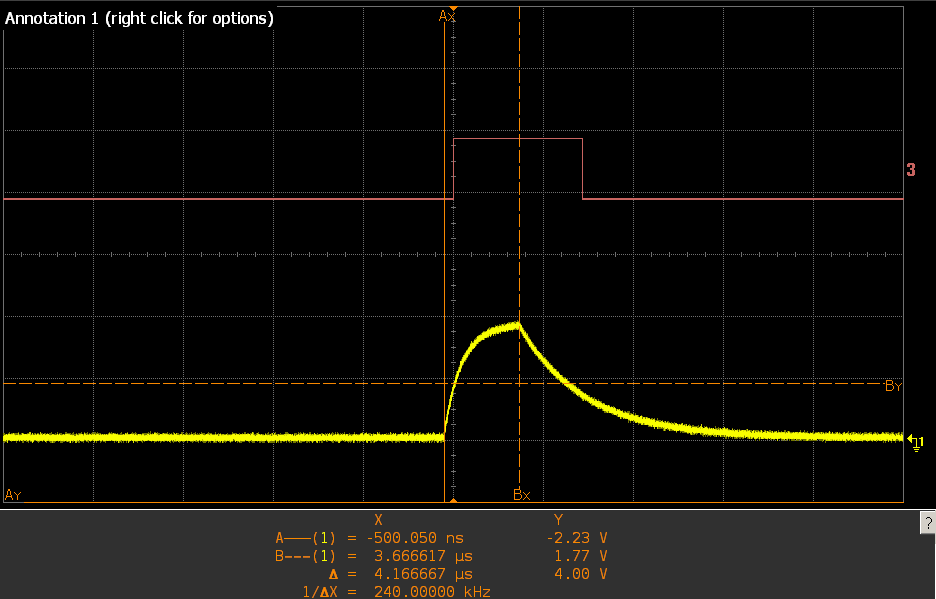
\includegraphics{pictures/messbild.png}}
 \caption{\label{impl_messbild} Reales und logisches Spannungsverhalten der Portpins}
\end{center}
 \textbf{Anmerkung:} In diesem Bild sind sowohl der reale Spannungsverlauf (gelb) als
 auch der logische Spannungsverlauf (rosa) auf der selben zeitlichen Basis dargestellt.
 Die horizontale braune Linie zeigt den Schwellenwert hat, ab dem der gemessene Portpin
 als logisch ''high'' betrachtet wird. Man erkennt hier auch deutlich, dass die Spannung
 beim zurücksetzen des Pins nur langsam abfällt.
\end{figure}

\section{Erste Messungen}
Durch die ersten Messungen wurde der Startpunkt für die Untersuchung der Software
festgelegt. Dafür wurde in der Hauptschleife (siehe Abb. \ref{main_loop_full}) zum einen
ein pin\_toggle() eingebaut, um die Länge einer Schleifeniteration zu messen; zum anderen
wurden die einzelnen Funktionsaufrufe in der Hauptschleife mit pin\_set() und pin\_clear()
umgeben.
\newcolumntype{R}{>{\raggedleft\arraybackslash}X}%
\begin{figure}[htb]
 \centering
 \scalebox{0.5}{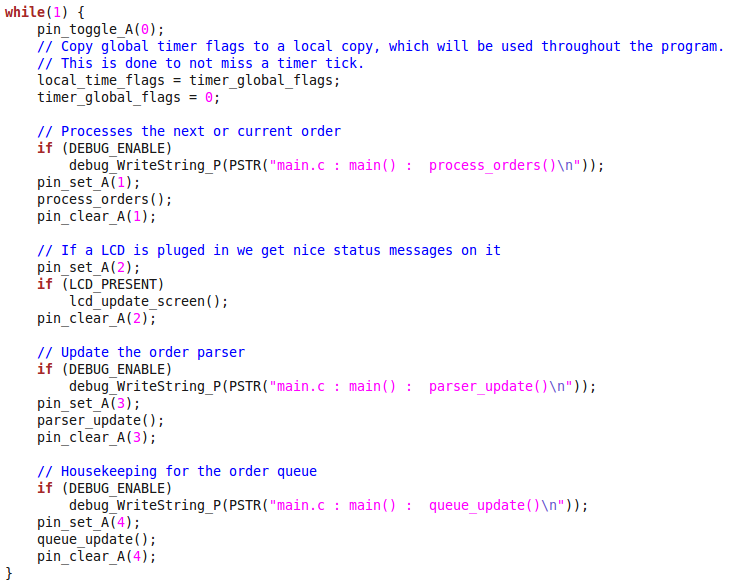
\includegraphics{pictures/main_loop_full.png}}
 \caption{\label{main_loop_full}Die Hauptschleife mit Debug-Ausgaben und Pin-Operationen}
\end{figure}
\begin{table}[htb]
\begin{center}
	\begin{tabular}{c}
	\begin{tabularx}{\textwidth}{|c||R|R|X|}
		\hline
		\textbf{Funktion}     & \textbf{vor der Code-Optimierung} & \textbf{nach der Code-Optimierung} & \textbf{Rahmen\-bedingungen} \\ 
		\hline \hline
		Hauptschleife         & 27,916 \textmu{}s      & 24,858 \textmu{}s       & Idle, LCD an, DEBUG aus, I2C an, AB:EIT \\ \hline
		process\_orders()     & 11,964 \textmu{}s      &  8,375 \textmu{}s       & \\ \hline
		lcd\_update\_screen() &  3,988 \textmu{}s      &  5,583 \textmu{}s       & \\ \hline
		parser\_update()      &  3,988 \textmu{}s      &  5,584 \textmu{}s       & \\ \hline
		queue\_update()       &  3,988 \textmu{}s      &  4,187 \textmu{}s       & \\ \hline
	\end{tabularx} \\
	\\
	\begin{tabularx}{\textwidth}{|c||R|R|X|}
		\hline
		Hauptschleife         & 47,856 \textmu{}s      & 42,473 \textmu{}s       & ABS aktiv im Idle-Status, ansonsten wie oben \\ \hline
		process\_orders()     & 31,904 \textmu{}s      & 26,221 \textmu{}s       & \\ \hline
		lcd\_update\_screen() &  3,988 \textmu{}s      &  5,484 \textmu{}s       & \\ \hline
		parser\_update()      &  3,988 \textmu{}s      &  5,683 \textmu{}s       & \\ \hline
		queue\_update()       &  3,988 \textmu{}s      &  4,686 \textmu{}s       & \\ \hline
	\end{tabularx} \\
	\\
	\begin{tabularx}{\textwidth}{|c||R|R|X|}
		\hline
		Hauptschleife         & 718,843 \textmu{}s     & 119,143 \textmu{}s      & LCD aus, Byte in Parser, Befehl bereit \\ \hline
		process\_orders()     &  39,880 \textmu{}s     &  18,544 \textmu{}s      & I2C-Bus-ISR (Daten) aufgetreten \\ \hline
		lcd\_update\_screen() &   0,997 \textmu{}s     &  $<$0,040 \textmu{}s      & \\ \hline
		parser\_update()      & 175,474 \textmu{}s     &  47,258 \textmu{}s      & \\ \hline
		queue\_update()       & 505,484 \textmu{}s     &  52,443 \textmu{}s      & \\ \hline
	\end{tabularx} \\
	\\
	\begin{tabularx}{\textwidth}{|c||R|R|X|}
		\hline
		Hauptschleife         & 3614,000 \textmu{}s    & 118,644 \textmu{}s      & LCD an, Befehl in Queue, \\
		                      &                        &                         & aber nicht gestartet \\ \hline
		process\_orders()     & 358,923 \textmu{}s     &  11,167 \textmu{}s      & \\ \hline
		lcd\_update\_screen() & 3250,000 \textmu{}s    &  97,109 \textmu{}s      & \\ \hline
		parser\_update()      & 6,032 \textmu{}s       &   5,783 \textmu{}s      & \\ \hline
		queue\_update()       & 5,583 \textmu{}s       &   3,988 \textmu{}s      & \\ \hline
	\end{tabularx} \\
	\\
	\begin{tabularx}{\textwidth}{|c||R|R|X|}
		\hline
		I2C-Bus-ISR           & 4,586 \textmu{}s       & 6,600 \textmu{}s        & Adresse empfangen \\ \hline
		I2C-Bus-ISR           & 21,934 \textmu{}s      & 6,600 \textmu{}s        & Daten empfangen \\ \hline
		100ms-ISR             & 8,076 \textmu{}s       & 5,583 \textmu{}s        & \\ \hline
	\end{tabularx} \\
	\end{tabular}
	\caption{\label{erste_messung} Ergebnisse der Messungen vor und nach den Code-Optimierungen}
\end{center}
\end{table}
In der Tabelle \ref{erste_messung} sind die wichtigsten Daten der ersten Messreihen zusammengefasst.
Die Spalte ''Rahmenbedingungen'' beschreibt Bedingungen, die während der Messung geherrscht haben.
Hierbei bezeichnet die Bedingung ''AB:EIT'', dass das aktive Bremsen (AB:) eingeschaltet (E; Enable) ist und
sowohl aktiviert wird, wenn kein Befehl bearbeitet wird (I; Idle), oder eines der Räder seinen Trigger früher
erreicht hat als das andere (T; Trigger). ''I2C an'' bezeichnet, dass der I2C-Bus für die E/A-Operationen
verwendet wurde und nicht die UART-Schnittstelle.\\
Interessant bei diesen Daten ist, dass das Aktualisieren der Warteschlange bei Vorliegen eines Befehls gut
eine halbe Millisekunde benötigt.

\section{Das LCD-Problem\label{chapter_lcd_problem}}
Wie in der Tabelle \ref{erste_messung} zu sehen ist, benötigt das System zum Aktualisieren der Informationen
des LCD über drei Millisekunden. Damit ist diese Funktion die mit Abstand zeitintensivste im gesamten System.
Das Aktualisieren erfolgt zwar recht selten, nämlich nur, wenn ein neuer Befehl gestartet wird; aber schon
bei drei Millisekunden Latenz wird die Reaktion des Systems auf Ereignisse negativ beeinflusst.
So könnten während der drei Millisekunden ungefähr zwölf Bytes auf dem I2C-Bus eintreffen.
Dies wären im schlimmsten Fall sechs eigenständige Befehle.
Wenn diese Befehle priorisierte Befehle sind, könnte sich das System anders verhalten als erwartet .\\
Zur Lösung dieses Problems musste die Arbeitsweise des LCD, welches durch eine fertige Programm-Bibliothek
gesteuert wird, analysiert werden. 
Dabei wurde herausgefunden, dass die Funktionen, die Daten auf das LCD ausgeben,
aktives Warten betreiben. Ein LCD benötigt natürlich Zeit, um ein übermitteltes Zeichen auch anzeigen zu können.
Während dieser Zeit wird das sog. Busy-Flag gesetzt, welches anzeigt, dass das LCD noch beschäftigt ist. Erst
wenn dieses Flag nicht mehr gesetzt ist, darf ein neues Zeichen übermittelt werden. Beim aktiven Warten verbraucht die
Funktion unnötig CPU-Zeit, die sinnvoll genutzt werden könnte.\\
Mit diesem Wissen wurde die ursprüngliche lcd\_\-update\_\-screen()-Funktion in zwei Funktionen aufgeteilt. Die eine
wurde lcd\_\-update\_\-info() genannt und aktualisiert die LCD-Informationen in einem Speicherpuffer. Die andere,
immer noch lcd\_\-update\_\-screen() genannt, überprüft das Busy-Flag des LCDs und schreibt das nächste Zeichen aus
dem Speicherpuffer aufs LCD, wenn es nicht gesetzt ist. Diese Lösung des Problems ist die effektivste, da die einzige
elegantere und effizientere die Benutzung eines Interrupts auf Basis des Busy-Flags wäre. Dies ist aber aufgrund der
Konstruktion des LCDs nicht möglich.
\begin{table}[htb]
\begin{center}
	\begin{tabular}{|c||r|r|c|}
		\hline
		\textbf{Funktion} & \textbf{Zeit} & \textbf{Verbesserung} & \textbf{Rahmenbedingungen} \\ \hline \hline
		Hauptschleife & 421,158 \textmu{}s & -88,35\% & LCD an, Befehl in Queue,\\
		& & & aber nicht gestartet \\ \hline
		process\_orders() & 354,627 \textmu{}s & & \\ \hline
		lcd\_update\_screen() & 57,884 \textmu{}s & -98,22\% & \\ \hline
	\end{tabular}
	\caption{\label{lcd_opt} LCD-Ergebnis}
\end{center}
\textbf{Anmerkung:} Für diese Tabelle und alle noch folgenden mit einer Rubrik ''Verbesserung'' gilt:\\
Prozentwerte der Verbesserung mit Minuszeichen bedeuten eine Reduzierung, mit Pluszeichen eine Erhöhung
der ursprünglichen Werte.
\end{table}
Wie in der Tabelle \ref{lcd_opt} zu sehen ist, hatten diese Maßnahmen aber ihre gewünschte Wirkung. Über 98\% weniger Zeit
wird nun im zeitintensivsten Fall benötigt. Die nachteillige Folge ist eine leicht erhöhte Laufzeit für das
Aktualisieren des LCD im Ruhezustand, deren Dauer sich von durchschnittlich 4 \textmu{}s auf 9 \textmu{}s erhöht hat.

\section{Optimierung}
Damit die Latenz des Systems möglichst niedrig ist, müssen die Funktionen, die in der Hauptschleife aufgerufen werden,
unter allen Bedingungen möglichst effizient ihre Arbeit verrichten. Dazu wurde jede dieser Funktionen mit dem 
''Pin-setzen-und-zurücksetzen-Verfahren'' auf Möglichkeiten untersucht, sie zu optimieren.

\subsection{Inlining von Funktionen}
Die erste Möglichkeit, die in Betracht gezogen wurde, um die Latenz des Systems zu verringern, war die Verwendung von
Compiler-Optimierungen. Zu Beginn wurde das System auf Code-Größe optimiert (-Os Option des Compilers). Da das System
wesentlich weniger Speicher benötigt, als auf der Platine zur Verfügung steht, wurde
anschließend der Compiler auf die Optimierung der Geschwindigkeit eingestellt (-O2 Option). Außerdem wurden die Debug-Informationen
(-g Option) entfernt, die der Compiler im Objektcode platziert hat. Dadurch änderten sich die Parameter des Systems nicht
wesentlich. Die Größe blieb nahezu identisch und die Geschwindigkeit stieg leicht an, besonders bei langen Funktionen.\\
Nachdem verifiziert werden konnte, dass Funktionsaufrufe zwischen 1 und 2 \textmu{}s Overhead mit sich bringen, wurde
die Compiler-Option -finline-functions aktiviert. Diese bewirkt, dass der Code von ausreichend simplen Funktionen direkt in die aufrufende
Funktion eingefügt wird, ohne dass dabei Register gerettet werden müssten oder Ähnliches. Dies hatte deutliche
Konsequenzen für die Geschwindigkeit des gesamten Systems, wie man in Tabelle \ref{compiler_flags_2} sehen kann.
\begin{table}[htb]
\begin{center}
	\begin{tabularx}{\textwidth}{|c||r|X|}
		\hline
		\textbf{Funktion} & \textbf{Zeit} & \textbf{Rahmenbedingungen} \\ \hline \hline
		Hauptschleife & 420,659 \textmu{}s & LCD an, Befehl in Queue,\\
		& & aber nicht gestartet, \\
		& & ohne -finline-functions \\ \hline
		process\_orders() & 355,289 \textmu{}s &  \\ \hline
		lcd\_update\_screen() & 59,481 \textmu{}s & \\ \hline
		parser\_update() & 4,146 \textmu{}s & \\ \hline
		queue\_update() & 4,640 \textmu{}s & \\ \hline \hline
	\end{tabularx}
	\begin{tabularx}{\textwidth}{|c||r|r|X|}
		\hline
		\textbf{Funktion} & \textbf{Zeit} & \textbf{Verbesserung} & \textbf{Rahmenbedingungen} \\ \hline \hline
		Hauptschleife & 285,643 \textmu{}s & -32,1\% & LCD an, Befehl in Queue,\\
		& & & aber nicht gestartet, \\
		& & & mit -finline-functions \\ \hline
		process\_orders() & 224,836 \textmu{}s & -36,72\% & \\ \hline
		lcd\_update\_screen() & 51,647 \textmu{}s & -13,17\% & \\ \hline
		parser\_update() & 5,384 \textmu{}s & +29,86\% & \\ \hline
		queue\_update() & 4,187 \textmu{}s & -9,76\% & \\ \hline
	\end{tabularx}
	\caption{\label{compiler_flags_2} Auswirkung von -finline-functions}
\end{center}
\end{table}

\subsection{Eliminierung von Modulo-Operatoren}
Während der Untersuchung der parser\_\-update()-Funktion wurde festgestellt, dass eine innere Funktion unverhältnismäßig
viel Zeit benötigt, um ihre Aufgabe zu erfüllen. Dies war die io\_\-get()-Funktion, deren Aufgabe es ist, das nächste Byte
im Eingangspuffer an den Aufrufer zurückzuliefern. Für diese simple Operation wurden über 36 \textmu{}s benötigt.
Das ist länger, als die gesamte Hauptschleife im Idle Zustand braucht.
Eine genaue Untersuchung der Funktion ließ darauf schließen, dass die Anweisungen
mit Modulo-Operatoren für diesen Aufwand verantwortlich waren. Das konnte zum einen durch Kontrolle des generierten
Assembler-Codes, zum anderen durch das Auslagern der Modulo-Operatoren in eine eigene Zeile bestätigt werden. Der Compiler generiert
für die Modulo-Operatoren eine Extra-Funktion, die sehr kompliziert ist und offensichtlich bemerkenswert viel Zeit benötigt.\\
\begin{verbatim}
uint8_t io_get(uint8_t* value) {
  pin_set_C(6);
  if ((inpos_begin + 1) % IO_INBUFFER_SIZE == inpos_end)
    return 0;
  pin_clear_C(6);
  pin_set_C(7);
  *value = in_buffer[inpos_begin];
  pin_clear_C(7);
  pin_set_C(1);
  inpos_begin = (inpos_begin + 1) % IO_INBUFFER_SIZE;
  pin_clear_C(1);
  return 1;
}
\end{verbatim}
Es gibt zwei Methoden, dies zu korrigieren: Zum einen kann die Modulo-Operation durch eine Reihe simplerer Operationen ersetzt werden.
Zum anderen kann auf die Modulo-Operation komplett verzichtet werden, wenn man das Überlaufverhalten der Variablen ausnutzen kann.
Die zweite Methode setzt voraus, dass der Puffer so viele Elemente hat, wie der größte darstellbare Wert der Variablen plus eins.
Da hier Variablen vom Typ uint8\_t verwendet werden (unsigned 8-bit integer bzw. vorzeichenlose 8-Bit-Ganzzahl) muss der Puffer 256
Elemente umfassen. Da diese Zahl bereits eingestellt war und diese Funktion sehr häufig verwendet wird, wurde hier die zweite Methode
benutzt. Es wurde dadurch nicht mehr Speicher verwendet als vorher, aber die Funktion lief daraufhin wesentlich schneller.
\begin{table}[htb]
\begin{center}
	\begin{tabular}{|l||r|r|}
		\hline
		\textbf{Funktion} & \textbf{Zeit} & \textbf{Verbesserung} \\ \hline \hline
		io\_get() & 36,527 \textmu{}s & \\ \hline
		io\_get() (umgeschrieben) & 3,393 \textmu{}s & -90,71\% \\ \hline
	\end{tabular}
	\caption{\label{io_get} Ergebnisse der io\_get()-Messungen}
\end{center}
\end{table}
Der Code sieht nun aus wie folgt:
\begin{verbatim}
uint8_t io_get(uint8_t* value) {
  uint8_t temp = (inpos_begin + 1);
  if (temp == inpos_end)
    return 0;
  *value = in_buffer[inpos_begin];
  inpos_begin = temp;
  return 1;
}
\end{verbatim}
Dasselbe Problem existierte in der Queue, dort wurden allerdings die Modulo-Operatoren
\begin{verbatim}
queue_writeposition %= QUEUE_SIZE;
\end{verbatim}
durch simplere Operationen ersetzt.
\begin{verbatim}
queue_writeposition -= (queue_writeposition
  / QUEUE_SIZE) * QUEUE_SIZE;
\end{verbatim}

\subsection{Effizienteres Initialisieren des Speichers}
Die Funktionen zum Initialisieren und Kopieren von Befehlen wurden wegen ihrer häufigen Verwendung ebenfalls
untersucht. Die Befehlsstrukturen wurden einfach mithilfe von Schleifen mit dem Wert 0 initialisiert, und beim
Kopieren wurden ebenfalls mit einer Schleife die Werte von einem Befehl in den nächsten kopiert. Diese Schleifen
wurden durch die memset()- bzw. die memcpy()-Funktion aus der Standardbibliothek ersetzt. Dies führte zu einem
40\%igen Geschwindigkeitszuwachs (siehe \ref{order_init_meas}).
\begin{table}[htb]
\begin{center}
	\begin{tabular}{|l||r|r|}
		\hline
		\textbf{Funktion} & \textbf{Zeit} & \textbf{Verbesserung} \\ \hline \hline
		order\_init() & 13,968 \textmu{}s & \\ \hline
		order\_init() (memset) & 7,976 \textmu{}s & -42,9\% \\ \hline
	\end{tabular}
	\caption{\label{order_init_meas} Ergebnisse der order\_init()-Optimierung}
\end{center}
\end{table}

\subsection{Bedingtes Kompilieren von Debug-Ausgaben}
Wie in Kapitel \ref{impl_debug} beschrieben, wurde eine Sprachen-spezifische Technik verwendet, um 
einfache Diagnoseausgaben zu ermöglichen, die im normalen Betrieb keine Auswirkung
auf das Laufzeitverhalten des Systems haben. So generiert der Compiler für die Ausgaben keinen Code, solange nicht
das Compilerflag -DDEBUG gegeben ist. Wenn es aber gegeben wurde, und die Ausgaben mithilfe des entsprechenden DIP-Schalters
deaktiviert sind, bringt jede Ausgabe lediglich eine Erhöhung der Laufzeit um weniger als eine \textmu{}s.

\section{Verlieren/Verpassen von Interrupts}
Während der Messungen kam die Frage auf, was passieren würde, wenn ein Interrupt auftritt und ein anderer bereits läuft.
Wenn dies möglich sein sollte, was geschieht dann mit den beiden Interrupts? Geht eventuell sogar einer davon verloren?\\
Die Antwort auf diese Fragen wurde von dem Handbuch des Mikrocontrollers \cite{ATMEGA_MANUAL} gegeben. Mit
den richtigen Einstellungen, die bereits vorgenommen wurden, werden Interrupts, die während eines anderen
Interrupts auftreten, gespeichert. Nach der Beendigung des laufenden Interrupts werden die anderen gespeicherten
ihrer Priorität nach ausgeführt.\\
Der schnellste Interrupt ist der UART-Interrupt. Er tritt maximal aller 138 \textmu{}s auf.
Im ungünstigsten Fall treten alle Interrupts zur selben
Zeit auf, und der danach am schnellsten wieder auftretende hat die niedrigste Priorität. Er wird also erst ausgeführt,
nachdem alle anderen Interrupts abgearbeitet wurden. Bei vier Hall-Sensoren-Interrupts, einem I2C-Bus-Interrupt,
einem Timer-Interrupt und zwei UART-Interrupts sowie einer oberen Schranke von 8 \textmu{}s pro Interrupt, plus
2 \textmu{}s Umschaltzeit zwischen zwei Interrupts, kommt man auf eine Zeit von 80 \textmu{}s.
Das bedeutet: Bevor der schnellste Interrupt wieder auftreten kann, wurden alle Interrupt-Service-Routinen
abgearbeitet und mindestens ein Hauptschleifendurchlauf beendet. Anzumerken ist hier noch, dass dieser konstruierte
ungünstigste Fall nicht möglich ist. Entweder ist der UART-Empfangs-Interrupt oder der I2C-Bus-Interrupt ausgeschaltet; sie
sind niemals zur selben Zeit aktiv. Außerdem benötigt der Großteil der Interrupts weniger als 5 \textmu{}s, um
seine Arbeit zu beenden. Hinzu kommt, dass die Hall-Sensoren-Interrupts, bedingt durch ihre Anordnung an den
Rädern, nicht alle zur selben Zeit auftreten können.\\
Die Hall-Sensoren-Interrupts treten sehr häufig auf, wenn die Räder in
Bewegung sind. Die Auswirkung dieser Interrupts auf das Echtzeitverhalten des Systems wurde daher
untersucht. Messungen ergaben, dass bei einer Spannung von 12 V und maximal
eingestellter Geschwindigkeit der Räder jeder Hall-Sensor aller 1,7 ms (d.s. 1700 \textmu{}s) einen Interrupt generiert.
Dieser Interrupt benötigt maximal 8 \textmu{}s. Während der 1700 \textmu{}s
treten insgesamt 4 Interrupts auf, jeweils einer pro Sensor; d.h. aller 425 \textmu{}s tritt ein Interrupt mit einer Länge
von 8 \textmu{}s auf. Somit werden zwischen zwei Interrupts der Hall-Sensoren im Durchschnitt 9 bis 10 Hauptschleifen-Iterationen
durchgeführt.

\section{Vergleich mit der Vorläufer-Software}
Der strenge Vergleich zwischen der Vorläufer-Software und der in dieser Arbeit geschriebenen Software ist
nur sehr bedingt möglich. Das zugrunde liegende Design von beiden Projekten ist so unterschiedlich, dass hauptsächlich
die Dauer der Hauptschleife andeuten kann, inwiefern die eine Software schneller arbeitet als die andere
(siehe Tabelle \ref{vergl_speed}).\\
Zusätzlich kann man noch den Speicherbedarf der Systeme vergleichen (siehe Tabelle \ref{vergl_speicher}). Hierbei
fällt auf, dass der generierte Maschinencode im Vergleich zum Vorläufer etwas größer ist. In Anbetracht
der benutzten Compiler-Flags bedeutet das aber, dass der Code mit gleichen Flags kleiner wäre als das Vorläufer. Dies ist
auch demonstriert worden, indem die Vorläufer-Software mit den Compiler-Flags der jetzigen Software übersetzt
wurde.
\begin{table}[htb]
\begin{center}
	\begin{tabular}{|l||r|}
		\hline
		\textbf{Speicherart} & \textbf{Belegung} \\ \hline \hline
		Program (Vorläufer) & 14968 Bytes (5,7\%)  \\ \hline
		Data (Vorläufer)& 1952 Bytes (23,8\%) \\ \hline \hline
		Program (Vorläufer + mod. Makefile) & 17808 Bytes (6,8\%)  \\ \hline
		Data (Vorläufer + mod. Makefile) & 1952 Bytes (23,8\%) \\ \hline \hline
		Program (aktuell)& 15362 Bytes (5,9\%) \\ \hline
		Data (aktuell)& 1248 Bytes (15,2\%) \\ \hline
	\end{tabular}
	\caption{\label{vergl_speicher} Vergleich der Speicheranforderung mit der Vorläufer-Software}
\end{center}
\end{table}
\begin{table}[htb]
\begin{center}
	\begin{tabular}{|l||r|r|c|}
		\hline
		\textbf{Funktion} & \textbf{Zeit} & \textbf{Verb.} & \textbf{Bedingung} \\ \hline \hline
		Hauptschleife (Vorläufer) & 121,885 \textmu{}s & & Idle \\ \hline
		Hauptschleife (mod. Vorl.) & 121,635 \textmu{}s & -0,21\% & Idle \\ \hline
		Hauptschleife (aktuell) & 23,535 \textmu{}s & -80,69\% & Idle \\ \hline \hline
		Befehl (kurz, Vorläufer) & 3655 \textmu{}s (13 Byte) & & I2C-Bus, kürzester Befehl \\ \hline
		Befehl (kurz, aktuell) & 1023 \textmu{}s (4 Byte) & & I2C-Bus, kürzester Befehl \\ \hline
		Befehl (lang, Vorläufer) & 7747 \textmu{}s (27 Byte) & & I2C-Bus, längster Befehl \\ \hline
		Befehl (lang, aktuell) & 2191 \textmu{}s (8 Byte) & & I2C-Bus, längster Befehl \\ \hline
	\end{tabular}
	\caption{\label{vergl_speed} Vergleich der Geschwindigkeiten mit der Vorläufer-Software}
\end{center}
\end{table}
Zusätzlich wurde noch verglichen, wie lange ein Befehl von der Praktikumsplatine bis zur Motorplatine benötigt.
Hier ist die Übertragungsgeschwindigkeit des I2C-Busses das größte Hindernis, aber dank der höheren Datendichte
der Befehlesübertragung im neuen System ist dieses wesentlich schneller (vgl. Tabelle \ref{vergl_speed} und Abb.
 \ref{vergl_befehle}).
\begin{figure}[htb]
\begin{center}
 \scalebox{0.35}{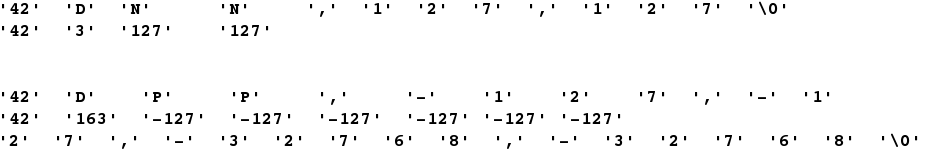
\includegraphics{pictures/vergl_befehle.png}}
 \caption{\label{vergl_befehle}Vergleich von mehreren Befehlen im alten und neuen Protokoll}
\end{center}
\textbf{Anmerkung:} Die vorliegende Abbildung zeigt sowohl den kürzesten als auch den längsten
Drive-Befehl im Format des alten und neuen Protokolls. Eine Zahl oder ein Buchstabe, der von ' eingeschlossen ist
repräsentiert den Wert eines Bytes. Dies verdeutlich die Reduktion der zu übertragenden Bytes
und die erhöhte Informationsdichte des neuen Protokolls.
\end{figure}
